\documentclass[12pt, oneside,a4paper, brazil]{abntex2}
% \documentclass[article,11pt,oneside,a4paper,twocolumn]{abntex2}
\usepackage[T1]{fontenc}
%\usepackage{natbib}
\usepackage[utf8]{inputenc}
\usepackage{indentfirst}
\usepackage{url}
\usepackage{xcolor}
\definecolor{verde}{rgb}{0.25,0.5,0.35}
\definecolor{jpurple}{rgb}{0.5,0,0.35}
\usepackage{listings}
\lstset{
  language=C++,
  basicstyle=\ttfamily\small,
  keywordstyle=\color{jpurple}\bfseries,
  stringstyle=\color{red},
  commentstyle=\color{verde},
  morecomment=[s][\color{blue}]{/**}{*/},
  extendedchars=true,
  showspaces=false,
  showstringspaces=false,
  numbers=left,
  numberstyle=\tiny,
  breaklines=true,
  backgroundcolor=\color{cyan!10},
  breakautoindent=true,
  captionpos=b,
  xleftmargin=0pt,
  tabsize=4
}
\pagestyle{empty}
\usepackage{lmodern}
\usepackage{epigraph}
\usepackage{microtype}
% \usepackage[brazilian,hyperpageref]{backref} Coloca na referência a página que está a citação
\usepackage[alf]{abntex2cite}	
\usepackage{graphicx}
\title{Relatório Final}
\instituicao{Universidade Federal do Rio Grande do Norte}
\local{Natal - RN}

\autor{Pedro Henrique Bezerra Cavalcante}
\date{\today}
\preambulo{Relatório final para obtenção parcial da nota da terceira unidade da disciplina Introdução à Ornanização e Arquitetura de Computadores do Bacharelado em Tecnologia da Informação, IMD/UFRN.}
\orientador{Mônica Magalhães Pereira}
\tipotrabalho{relatorio}
\setlrmarginsandblock{3cm}{3cm}{*}
\setulmarginsandblock{3cm}{3cm}{*}
\setlength{\parindent}{1.25cm} %Funcionou 
\SingleSpacing

\begin{document}
\selectlanguage{brazil}

\frenchspacing
\imprimircapa
\imprimirfolhaderosto

\tableofcontents
\chapter{Introdução}
\section{Daisy Chaining}
A Arbitragem por Daisy Chain tem como vantagem a simplicidade de implemetação. Por outro lado, é desvantajoso pelo motivo de que ``um dispositivo de menor prioridade pode não conseguir acesso ao barramento''\cite{Silva}, podendo ficar, assim, bloqueado indefinidamente. O uso desse esquema de arbitragem ``também limita a velocidade do barramento''\cite{Silva}. 	
\section{Prioridade}
A forma de árbitrariedade por prioridade é executada de acordo com a prioridade inerente ao dispositivo que solicitou execução. 
\section{Justiça}
Arbritrariedade por tempo de justiça é dada da forma que: cada dispositivo tem seu tempo de execução. Por justiça, o árbitro é implementado com um tempo fixo de execução. Caso o dispositivo leve mais tempo que o árbitro permite, ele é executado, interrompido e passa para o final da linha de execução. Dessa forma, 


%\chapter{Material Utilizado}
\chapter{Descrição e Organização do Projeto e Execução}
O projeto foi desenvolvido em linguagem C++ e está distribuído em três arquivos:
\begin{enumerate}
	\item main.cpp: contem a função principal do projeto
	\item perifericos.h: contem os cabeçalhos de funções do projeto
	\item perifericos.cpp: contém a implementação das funções.
\end{enumerate}
Deve ser executado através do comando: 
\begin{lstlisting}
g++ -Wall main.cpp perifericos.cpp -o <arquivo de saida>
\end{lstlisting}

A primeira parte do programa irá solicitar a entrada do usuário para definir quantos periféricos irão solicitar execução. 
\begin{figure}[!htb]
\centering
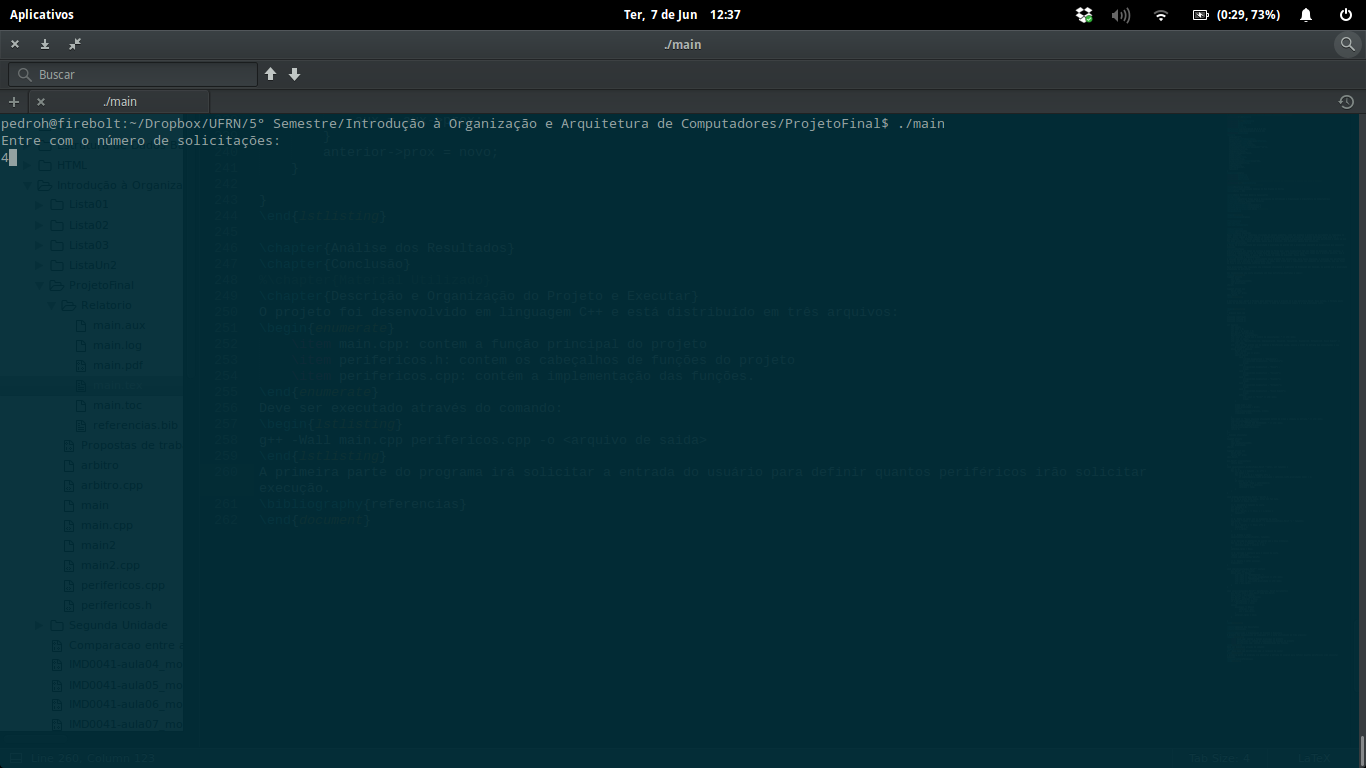
\includegraphics[scale=0.3]{img1.png}
\caption{Exemplo de entrada para quantidade de periféricos}
\label{Gráfico 1}
\end{figure}

Em seguida, irá solicitar ao usuário que entre com o ńúmero correspondente ao dispositivo e sua respectiva prioridade, como se pode ver na imagem a seguir:
\begin{figure}[!htb]
\centering
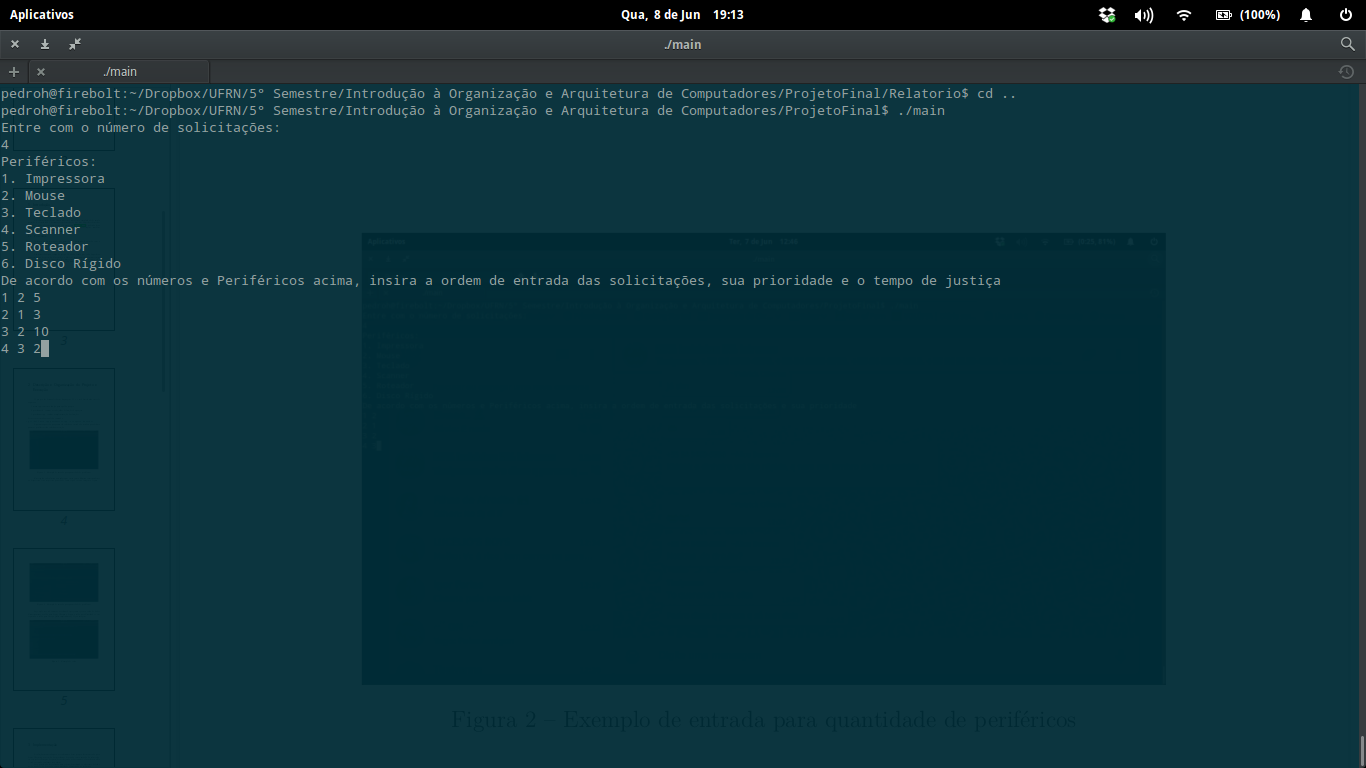
\includegraphics[scale=0.3]{img2.png}
\caption{Exemplo de entrada para os periféricos, sua prioridade e seu tempo de execução}
\label{Gráfico 1}
\end{figure}
\newpage
Logo após isso, irá executar as rotinas do programa e gerar a saída de dados. Primeiramente a saída para Daisy Chaining, depois a saída para Prioridade e, em seguinda, a saída para Justiça (falta implementar). Veja a imagem.
\begin{figure}[!htb]
\centering
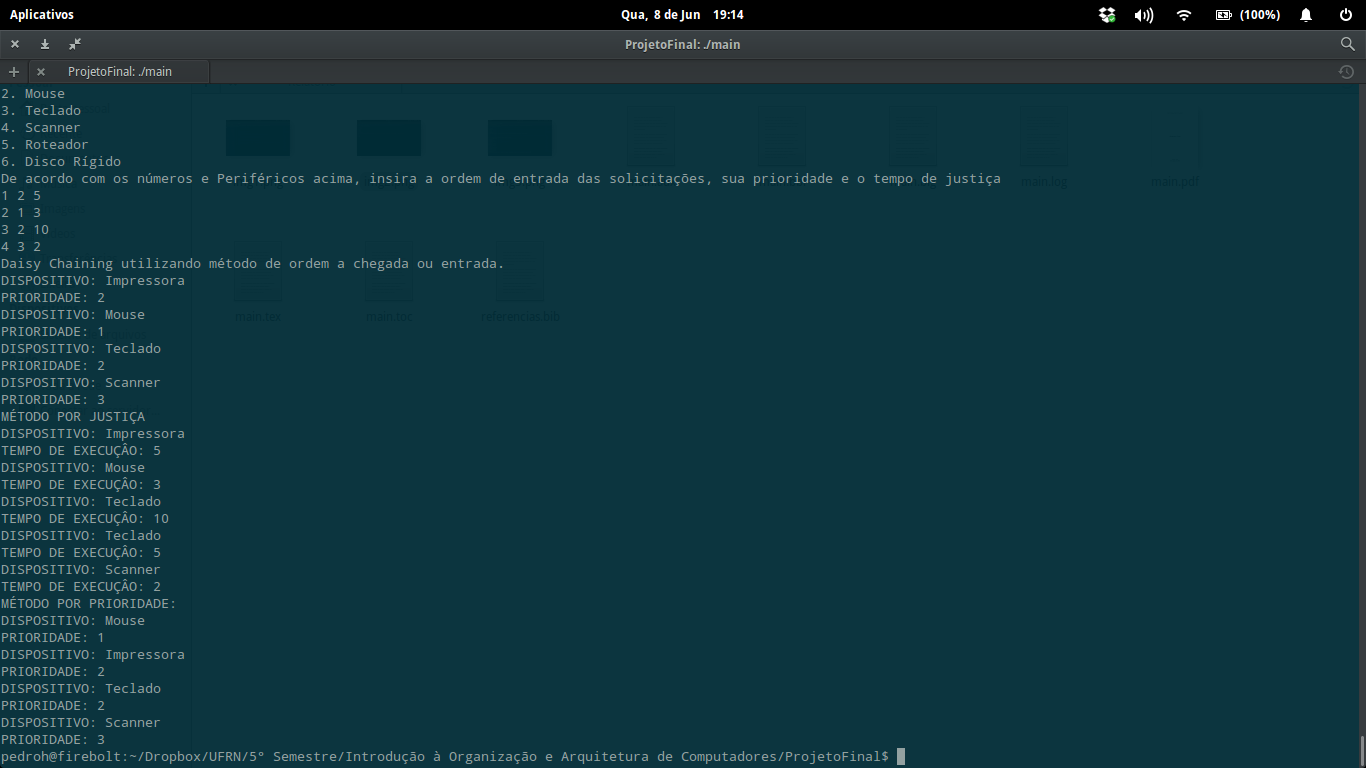
\includegraphics[scale=0.3]{img3.png}
\caption{Exemplo de saída}
\label{Gráfico 1}
\end{figure}
\chapter{Implementação}
A solução encontrada para o resolvimento desse projeto foi encontrada, para Daisy Chaining, a execução dos periféricos de acordo com a entrada da solicitação, ou seja, pelo ordem que a requisição vai chegando ao barramento, ela vai ficar na fila e será executada conforme essa ordem. 

Para prioridade, foi realizada uma ordenação utilizando o algoritmo de Ordenação por Seleção, de acordo com a prioridade armazenada na estrutura. 

Foi desenvolvida uma lista encadeada com duas estruturas,mostradas à seguir: 
\begin{lstlisting}
typedef struct{
	int tipo;
	char dispositivo[50];
	int prioridade;
}Perif;

typedef struct no{
	Perif info;
	struct no* prox;
}Aux_Perif;
\end{lstlisting}

A estrutura Aux\_perif é formada pelo ponteiro para o próximo no e uma estrutura Perif. Essa última, é formada pelos dados do periférico, que é seu tipo (int), o nome do dispositivo (char) e a sua prioridade (int).


\begin{lstlisting}
/**
* Arquivo main.cpp
*/
#include <iostream>
#include <string.h>
#include <stdlib.h>
#include "perifericos.h"


int main(){
	int solic;
	int cont = 0;
	int justica = 0;
	int aux = 0, prior = 0;
	Aux_Perif* perifericos;
	Aux_Perif* perif_just;
	perifericos = criarLista();
	perif_just = criarLista();
	std::cout << "Entre com o numero de solicitacoes: " << std::endl;
	std::cin >> solic;
	std::cout << "Perifericos:\n1. Impressora\n2. Mouse\n3. Teclado\n4. Scanner\n5. Roteador\n6. Disco Rigido" << std::endl;
	std::cout << "De acordo com os numeros e Perifericos acima, insira a ordem de entrada das solicitacoes, sua prioridade e o tempo de justica" << std::endl;
	while (cont < solic){
		Perif ordem;
		Perif justica_vet;
		std::cin >> aux >> prior >> justica;
		switch (aux){
			case 1:
				//ordem.dispositivo = 'Impressora';
				strcpy(ordem.dispositivo, "Impressora");
				strcpy(justica_vet.dispositivo, "Impressora");
				break;
			case 2: 
				strcpy(ordem.dispositivo , "Mouse") ;
				strcpy(justica_vet.dispositivo, "Mouse");
				break;
			case 3: 
				strcpy(ordem.dispositivo , "Teclado");
				strcpy(justica_vet.dispositivo, "Teclado");
				break;
			case 4:
				strcpy(ordem.dispositivo , "Scanner");
				strcpy(justica_vet.dispositivo, "Scanner");
				break;
			case 5:
				strcpy(ordem.dispositivo , "Roteador");
				strcpy(justica_vet.dispositivo, "Roteador");
				break;
			case 6: 
				strcpy(ordem.dispositivo , "Disco Rigido");
				strcpy(justica_vet.dispositivo, "Disco Rigido");
				break;
			default:
				std::cout << "Error" << std::endl;
				break;
		}
		
		ordem.tipo = aux;
		justica_vet.tipo = aux;

		ordem.prioridade = prior;
		justica_vet.prioridade = prior;

		justica_vet.set_used = true;
		ordem.set_used = true;

		ordem.justica = justica;
		justica_vet.justica = justica;

		cont++;
		inserirFinal(&perifericos, ordem);
		inserirFinal(&perif_just, justica_vet);
	}
	std::cout << "Daisy Chaining utilizando metodo de ordem a chegada ou entrada." << std::endl;
	imprimirLista(&perifericos);
	std::cout << "METODO POR JUSTICA" << std::endl;
	imprimirLista_Justica(&perif_just);
	std::cout << "METODO POR PRIORIDADE: " << std::endl;
	ordena_AuxPerif(&perifericos);
	imprimirLista(&perifericos);
	return 0;
}

	
}
/**
* Arquivo perifericos.h
*/
#ifndef _PERIFERICOS_H_
#define _PERIFERICOS_H_

#include <iostream>
#include <string.h>
#include <stdlib.h>

typedef struct{
	int tipo;
	char dispositivo[50];
	int prioridade;
	int justica;
	bool set_used = false;
}Perif;

typedef struct no{
	Perif info;
	struct no* prox;
}Aux_Perif;

Aux_Perif* criarLista();
void selectionsort_AuxPerif(Aux_Perif **vetor, int tamanho);
void ordena_AuxPerif(Aux_Perif **perif);
void imprimirLista(Aux_Perif** lista);
void inserirFinal(Aux_Perif** perifericos, Perif barramento);
void percorre_true(Aux_Perif** lista, int dispo, int prioridade);
void imprimirLista_Justica(Aux_Perif** lista);

#endif


/**
* Arquivo perifericos.cpp
*/

#include <iostream>
#include <string.h>
#include <stdlib.h>
#include "perifericos.h"

Aux_Perif* criarLista(){
	return NULL;
}

void selectionsort_AuxPerif(Aux_Perif **vetor, int tamanho) {
    int i, j;
    for (i = 0; i < tamanho - 1; i++) {
        int menor = i;
        for (j = i + 1; j < tamanho; j++) {
            if (vetor[menor]->info.prioridade > vetor[j]->info.prioridade) menor = j;
        }
        if (menor != i) {
            Aux_Perif *temp = vetor[menor];
            vetor[menor] = vetor[i];
            vetor[i] = temp;
        }
    }
}

void ordena_AuxPerif(Aux_Perif **perif) {
    // 1. Se a lista esta vazia, entao nem faz nada.
    if (perif == NULL) return;

    // 2. Descobre o tamanho da lista.
    int tamanho = 0;
    Aux_Perif *v;
    for (v = *perif; v != NULL; v = v->prox) {
        tamanho++;
    }

    // 3. Monta um vetor com os elementos da lista.
    Aux_Perif **vetor = (Aux_Perif **) malloc(sizeof(Aux_Perif *) * tamanho);
    int i = 0;
    for (v = *perif; v != NULL; i++) {
        vetor[i] = v;
        v = v->prox;
    }

    // 4. Ordena o vetor.
    selectionsort_AuxPerif(vetor, tamanho);

    // 5. Corrige os ponteiros de acordo com a nova ordenacao.
    for (i = 0; i < tamanho - 1; i++) {
        vetor[i]->prox = vetor[i + 1];
    }
    vetor[i]->prox = NULL;

    // 6. Corrige o ponteiro para o inicio da lista.
    *perif = vetor[0];
    //void imprimirLista(*perif);

    // 7. Deleta o vetor auxiliar.
    free(vetor);
}

void imprimirLista(Aux_Perif** lista){
	Aux_Perif* aux = *lista;
	while (aux != NULL && aux->info.set_used == true){
    //while (aux != NULL){
		std::cout << "DISPOSITIVO: ";
		std::cout << aux->info.dispositivo << std::endl;
		std::cout << "PRIORIDADE: ";
		std::cout << aux->info.prioridade << std::endl;
		aux = aux->prox;
	}
}

void imprimirLista_Justica(Aux_Perif** lista){
    Aux_Perif* aux = *lista;
    while(aux != NULL){
        int teste = aux->info.justica;
        while(teste > 0){
            std::cout << "DISPOSITIVO: ";
            std::cout << aux->info.dispositivo << std::endl;
            std::cout << "TEMPO DE EXECUCAO: ";
            std::cout << teste << std::endl;
            teste = teste-5;
        }
        aux = aux->prox;
    }
}

void inserirFinal(Aux_Perif** perifericos, Perif barramento){
	Aux_Perif* novo = (Aux_Perif*)new Aux_Perif;
	novo->info = barramento;
	Aux_Perif* aux = *perifericos;
	Aux_Perif* anterior = NULL;
	if (*perifericos == NULL){
		*perifericos = novo;
	}else{
		while(aux != NULL){
			anterior = aux;
			aux = aux->prox;
		}
		anterior->prox = novo;
	}

}

void percorre_true(Aux_Perif** lista, int dispo, int prioridade){
    Aux_Perif* aux = *lista;
    while (aux != NULL){

        if (aux->info.tipo == dispo){
            aux->info.set_used = true;
            aux->info.prioridade = prioridade;   
        }else{
            aux->info.prioridade = prioridade;

         
        }
        aux = aux->prox;   
    }
}
\end{lstlisting}

\chapter{Análise dos Resultados}
\chapter{Conclusão}

\bibliography{referencias}
\end{document}